\chapter{Antecedentes}
\section{Antecedentes y contextualización del neurodesarrollo infantil}
\subsection{Panorama global del desarrollo infantil}
A nivel global, los desafíos asociados con el desarrollo infantil son amplios 
y están influenciados por múltiples factores socioeconómicos, culturales y 
ambientales. Según UNICEF, aproximadamente 250 millones de niños menores de 5 
años se encuentran en riesgo de no alcanzar su potencial de desarrollo debido 
a factores como la desnutrición, la falta de estimulación temprana y el acceso 
limitado a servicios de salud y educación \cite{UNICEF2023}. Estas condiciones 
adversas son particularmente prevalentes en países de ingresos bajos y medios, 
donde se observan altas tasas de desnutrición crónica y pobreza infantil.

La neurociencia del desarrollo ha demostrado que los primeros años de vida, 
especialmente los primeros 1000 días, son críticos para el desarrollo cerebral 
óptimo. Durante este período, las experiencias ambientales y las interacciones 
con los cuidadores moldean la arquitectura neural, determinando habilidades 
fundamentales como el lenguaje, la memoria y el control emocional 
\cite{Stiles2010}. Las adversidades tempranas, incluyendo la pobreza y la 
desnutrición, pueden generar efectos negativos duraderos en la plasticidad 
cerebral, lo que subraya la importancia crítica de intervenciones tempranas y 
programas de estimulación adecuados.

Desde una perspectiva bioecológica, el desarrollo infantil está influenciado 
por diversos niveles contextuales que interactúan dinámicamente entre sí, como 
se describe en el modelo de Bronfenbrenner \cite{Bronfenbrenner2005}. Este 
enfoque destaca la relevancia de los entornos inmediatos, como la familia y la 
comunidad, así como de factores contextuales más amplios, incluyendo las 
políticas públicas y las normas culturales. En Guatemala, el acceso limitado a 
programas de primera infancia y los altos índices de desnutrición crónica 
restringen significativamente las oportunidades de desarrollo infantil, 
especialmente en comunidades rurales e indígenas \cite{SESAN2022}.

\subsection{Contexto guatemalteco del neurodesarrollo infantil}
Guatemala se caracteriza por su rica diversidad cultural, conformada por 
cuatro grupos étnicos principales: Maya, Garífuna, Xinka y Mestizo. Aunque la 
mayoría de la población guatemalteca (54\%) reside en zonas urbanas, es 
importante señalar que la población indígena habita predominantemente en áreas 
rurales (57\%) \cite{PoliticaInfanciaGuate}.

El panorama demográfico de Guatemala presenta importantes desafíos para la 
primera infancia. Según datos del censo poblacional de 2018, en el país 
habitan aproximadamente 2.3 millones de niñas y niños menores de 6 años, de 
los cuales cerca de 1 millón viven en condiciones de pobreza y 800 mil en 
situación de pobreza extrema \cite{INE}. Los departamentos con mayor proporción 
de población infantil temprana son Totonicapán (41.7\%), Huehuetenango (41.4\%) 
y El Quiché (41.1\%) \cite{UNICEFAtlas}. Adicionalmente, el 3.8\% de la 
población infantil y adolescente entre 4 y 17 años presenta algún tipo de 
dificultad visual, auditiva, física, de concentración, autocuidado o 
comunicación \cite{INE}.

Si bien Guatemala constituye la economía más grande de América Central en
términos de población (aproximadamente 17.6 millones de habitantes en 2023) y
actividad económica (con un PIB de 104.4 mil millones de dólares
estadounidenses en 2023), este crecimiento económico no se ha traducido en una
reducción significativa de la pobreza. Para 2023, se estimaba que el 55\% de la
población vivía en condiciones de pobreza, mientras que la economía informal
representaba el 49\% del PIB, con un 71.1\% de la población empleada trabajando
en el sector informal \cite{WorldBankGuate}. Es importante destacar que la
pobreza y las experiencias adversas durante la infancia tienen efectos
fisiológicos y epigenéticos a largo plazo en el desarrollo cerebral y la
cognición \cite{Luby_2015, Noble_2015}.

La situación del desarrollo infantil en Guatemala es preocupante. De acuerdo
con los datos de 2021-2022, Guatemala ha obtenido un 49.8\% en el Índice de
Desarrollo Infantil Temprano, lo que significa que menos de la mitad de los
niños entre 24 y 59 meses presenta un desarrollo adecuado en salud, aprendizaje
y bienestar psicosocial. Existen disparidades significativas entre diferentes
grupos poblacionales: mientras que el 57.9\% de los niños no indígenas muestra
un desarrollo adecuado, solo el 45\% de los niños indígenas alcanza este nivel
\cite{SESAN2022}. Las diferencias se acentúan aún más cuando se analiza el
índice en función de la riqueza del hogar, observándose una brecha de 23 puntos
porcentuales entre los hogares con mayor y menor riqueza \cite{UNICEFGuate}.

El limitado acceso a oportunidades educativas constituye otro desafío 
fundamental. En 2020, la tasa neta de cobertura en el nivel inicial fue de 
apenas el 1.1\% a nivel nacional. En ese mismo año, se registraron 597,195 
niñas y niños inscritos en educación preprimaria, con una cobertura nacional 
del 60.8\%, representando el 13.8\% del total de estudiantes inscritos en los 
distintos niveles educativos \cite{PoliticaInfanciaGuate}. Para niños menores 
de 4 años, la cobertura educativa es particularmente baja, mientras que para 
niños entre 4 y 6 años alcanza el 64.4\% \cite{MineducEstadistica}.

La situación educativa de la niñez con discapacidad representa un desafío
particular para el país. Según la Encuesta Nacional de Discapacidad en Guatemala
de 2016, el 76\% de las niñas y niños entre 5 y 18 años con algún tipo de
discapacidad asiste a la escuela, observándose una marcada diferencia entre el
área urbana (90\%) y el área rural (61\%). Los niños con limitaciones
significativas en el funcionamiento físico o cognitivo tienen menor probabilidad de ser inscritos en establecimientos educativos \cite{PoliticaInfanciaGuate}.

Al analizar la relación entre desarrollo infantil temprano y estado nutricional, 
los resultados son consistentes con estudios previos que demuestran que los 
niños con desnutrición crónica tienden a presentar menor desarrollo. En la 
encuesta de línea base de la Cruzada Nacional por la Nutrición 2021/2022, esta 
relación se evidencia claramente: el porcentaje de niños con desarrollo 
adecuado es mayor entre aquellos que no presentan desnutrición crónica (55.6\%) 
en comparación con quienes padecen este tipo de malnutrición (43.3\%) 
\cite{SESAN2022}.

La desnutrición crónica afecta aproximadamente al 46.5\% de los niños
guatemaltecos menores de 5 años, reflejando profundas desigualdades sociales.
El porcentaje de desnutrición crónica es significativamente mayor en áreas
rurales (53\% frente a 34.6\% en zonas urbanas), en población indígena (58\%
frente a 34.2\% en población no indígena), en hogares donde las madres carecen
de escolaridad (67.0\% frente a 19.1\% en hogares donde la madre tiene
educación superior), en hogares con menor riqueza económica (65.9\% en el
quintil inferior frente a 17.4\% en el quintil superior) y cuando existe menor
espaciamiento entre embarazos (57.0\% frente a 39.6\% con mayor espaciamiento)
\cite{EnMaternoInfantil}.

Las prácticas de alimentación infantil también presentan importantes desafíos.
Solo el 63.1\% de las niñas y niños reciben lactancia materna dentro de la
primera hora de nacidos, el 53.2\% reciben lactancia materna exclusiva entre
los 0 y 6 meses de edad, y la duración promedio de la lactancia materna
exclusiva es de apenas 2.8 meses. En cuanto a la alimentación complementaria,
el 55.7\% de los niños entre 6 y 23 meses que son amamantados reciben cuatro o
más grupos de alimentos, mientras que el 71.2\% de los niños no amamantados en
este mismo rango de edad reciben una frecuencia mínima de comidas
\cite{EnMaternoInfantil, PoliticaInfanciaGuate}.

Si bien la calidad del vínculo entre cuidadores y niños constituye un factor
fundamental para el desarrollo infantil óptimo, las estadísticas en Guatemala
revelan un patrón preocupante de violencia ejercida por los cuidadores hacia
los niños bajo su responsabilidad. Un estudio realizado a finales de 2019 en 52
comunidades de los departamentos de Sololá, Alta Verapaz, Baja Verapaz,
Chimaltenango, Quetzaltenango y San Marcos reveló que 8 de cada 10 adultos
consideran que en su comunidad la forma más habitual de corregir a los hijos es
mediante castigos físicos como cincho, chicote, vara, golpes o gritos. La mitad
de los adultos piensa que la falta de este tipo de disciplina refleja una
carencia de carácter por parte de los padres
\cite{PoliticaInfanciaGuate, UNICEFComportamientosNinez}.

\subsection{Estudios previos sobre factores de riesgo en el neurodesarrollo}
En una revisión sistemática y metaanálisis realizada por Wondmagegn et al.
(2024), titulada ``Prevalencia y determinantes del retraso del desarrollo entre
los niños en países de ingresos bajos y medios: una revisión sistemática y un
metaanálisis'', se analizaron 21 estudios primarios publicados entre 2010 y
2024, involucrando a un total de 54,067 niños en países de ingresos bajos y
medios. El objetivo principal fue evaluar la prevalencia combinada del retraso
del desarrollo confirmado y sus determinantes entre los niños en estos países.
Los resultados mostraron una prevalencia combinada de retraso del desarrollo
del 18.83\% (IC 95\%: 15.53-22.12\%). En el análisis de subgrupos, se observó
una alta prevalencia de retraso del desarrollo [26.69\% (IC 95\%: 15.78-37.60)]
en estudios realizados en África. Los determinantes significativos del retraso
del desarrollo fueron la educación materna [OR: 3.04; IC 95\% (2.05, 4.52)] y
el bajo peso al nacer [OR: 3.61; IC 95\% (1.72, 7.57)]. Los autores concluyeron
que la prevalencia combinada de retraso del desarrollo en países de ingresos
bajos y medios era alta en comparación con los países de altos ingresos,
especialmente en África, y que el nivel educativo materno y el peso al nacer
estaban significativamente asociados con los retrasos del desarrollo
\cite{Wondmagegn2024}.

En un estudio transversal realizado por Mehner et al. (2019), titulado
``La asociación de la puntuación de riesgo acumulativo con los resultados de
ASQ-3 en una región rural empobrecida de Guatemala'', se evaluó una muestra de
conveniencia de 148 madres con niños de 12 a 52 meses de edad en una zona rural
de Guatemala. El objetivo principal fue desarrollar una puntuación de riesgo
compuesta por factores fácilmente obtenibles para diseñar intervenciones e
identificar a los niños de alto riesgo que más se beneficiarían de estas. Se
utilizaron encuestas de interacción madre-hijo y \asq\ para evaluar el
desarrollo. Los resultados mostraron que el 58\% de los niños tenían
puntuaciones anormales en $\ge$1 dominio del ASQ-3, y el 35\% en $\ge$2
dominios. Se desarrollaron tres puntuaciones de riesgo: Riesgo Demográfico
Materno (DR), Interacción Madre-Hijo (MCI) y Riesgo Combinado (CR). La
probabilidad de tener $\ge$2 dominios con puntuaciones anormales aumentó
significativamente con un puntaje DR creciente (OR, 1.46 [IC 95\%, 1.15-1.86]
p<0.05) y un puntaje CR creciente (OR, 2.08 [IC 95\%, 1.41-3.07], p<0.05). Los
autores concluyeron que un índice de riesgo acumulativo combinado de factores
demográficos e interacciones madre-hijo parece ser una herramienta útil para
predecir qué niños tienen puntuaciones anormales en múltiples dominios del
desarrollo \cite{CMehner2019}.

En el contexto específico de Guatemala, un análisis del informe de la  línea de
base de la Gran Cruzada Nacional por la Nutrición 2021/2022 revela  datos
preocupantes: la cobertura de programas de primera infancia es extremadamente
limitada, con apenas un 1.9\% de niños entre 2 y 5 años que han asistido alguna
vez a estos programas. Más alarmante aún es que solo el 49.8\% de los niños
guatemaltecos entre 24 y 59 meses muestran un desarrollo adecuado  en las
dimensiones de salud, aprendizaje y bienestar psicosocial \cite{SESAN2022}.
Estos datos son consistentes con las observaciones de Mehner et al.
\cite{CMehner2019} en zonas rurales de Guatemala, donde encontraron que el 58\%
de los niños evaluados presentaban puntuaciones anormales en al menos un
dominio del ASQ-3.

\subsection{Brechas en el conocimiento e importancia del estudio actual}
En el distrito de Quetzaltenango, Guatemala, la vulnerabilidad económica, el
acceso limitado a servicios de salud y los factores nutricionales representan
riesgos significativos para el neurodesarrollo infantil. Al igual que en otros
países de ingresos bajos y medios, las condiciones adversas en esta región
pueden influir negativamente en los hitos del desarrollo infantil temprano.

Esta problemática local se enmarca en un contexto global igualmente 
preocupante. Según UNICEF \cite{UNICEF2023}, aproximadamente 250 millones de 
niños menores de 5 años a nivel mundial están en riesgo de no alcanzar su 
potencial de desarrollo, con cerca de 200 millones afectados por desnutrición 
en la primera infancia. Particularmente relevante para este estudio es que más
de 2 de cada 5 niños entre 3 y 4 años no reciben la estimulación temprana ni el
cuidado parental adecuados, factores que Domek et al. \cite{Domek2023} 
identificaron como críticos para el desarrollo socioemocional y del lenguaje. 

La unión de los datos nacionales con los hallazgos globales subraya la 
necesidad de investigaciones específicas en contextos como Quetzaltenango, 
donde factores socioeconómicos, nutricionales y de acceso a servicios de salud 
pueden influir significativamente en los patrones de desarrollo infantil.

\section{Neurodesarrollo: Definición y relevancia}
El neurodesarrollo es un proceso dinámico y continuo que se extiende desde 
las primeras etapas de la vida intrauterina hasta la adultez, abarcando una 
compleja interacción de factores genéticos, epigenéticos, ambientales y 
sociales. Este proceso es fundamental para el establecimiento de las bases 
cognitivas, emocionales, motoras y sociales de los individuos, las cuales 
son esenciales para su aprendizaje, adaptación y productividad a lo largo 
de la vida \cite{Stiles2010, Nelson49}.

El desarrollo cerebral está regulado por una interacción entre la expresión 
genética y las influencias ambientales. Mientras que los genes proporcionan 
el marco básico para el desarrollo de estructuras neuronales, las 
experiencias tempranas y las interacciones sociales desempeñan un papel 
crítico en la modelación de las conexiones sinápticas y en la poda neuronal. 
Como señala Stiles \cite{Stiles2010}, ``tanto la expresión genética como los
estímulos ambientales son esenciales para el desarrollo cerebral normal, y la
alteración de cualquiera de estos factores puede modificar fundamentalmente los
resultados neurales''. Estos mecanismos epigenéticos, como la metilación del
ADN, permiten que el entorno modifique la expresión genética sin alterar la
secuencia del ADN,  impactando así el desarrollo cerebral y la consolidación de
habilidades cognitivas y emocionales \cite{Roth2011, Feldman2}.

En el aspecto biológico, el neurodesarrollo durante los primeros años de vida
representa un período crítico caracterizado por un desarrollo acelerado, 
durante el cual numerosas estructuras neuronales se construyen y organizan 
siguiendo las siete fases fundamentales del desarrollo cerebral: nacimiento 
celular, migración celular, diferenciación celular, maduración celular, 
sinaptogénesis, muerte celular y poda sináptica, y mielinización.
\cite{Kolb7}

El neurodesarrollo abarca diversos dominios neurológicos fundamentales que 
evolucionan siguiendo trayectorias interconectadas: sensorial, motor grueso y
fino, lingüístico, visuo-espacial, intelectual, memoria, cognición social y
función ejecutiva. La maduración de estos dominios sigue una secuencia
relativamente predecible, aunque con  variaciones individuales significativas,
que se manifiesta a través de la  adquisición de habilidades cada vez más
complejas y refinadas. \cite{Nelson49}

\subsection{Relevancia del neurodesarrollo infantil}
El neurodesarrollo infantil tiene repercusiones tanto individuales como
colectivas, siendo un aspecto clave para la salud pública. Las investigaciones
muestran que retrasos en el neurodesarrollo están asociados con una mayor carga
económica y social, debido a la necesidad de intervenciones educativas, médicas
y sociales.

El neurodesarrollo infantil también está intrínsecamente ligado a las 
desigualdades sociales y económicas. Los niños que viven en condiciones de 
pobreza enfrentan una mayor probabilidad de exposición a factores de riesgo, 
como la desnutrición y la falta de estimulación temprana. Estas desigualdades 
no solo limitan el potencial individual, sino que perpetúan el ciclo de pobreza 
entre generaciones. \cite{UNICEF2023}

Las intervenciones tempranas han demostrado ser una estrategia efectiva para 
mitigar los efectos negativos en el neurodesarrollo. Estas intervenciones
incluyen programas de estimulación temprana, atención prenatal y postnatal de
calidad, y políticas públicas que promuevan el acceso a una nutrición adecuada
y a servicios educativos.

\section{Procesos biológicos del desarrollo cerebral}
El cerebro humano evoluciona a partir de un grupo limitado de células
embrionarias hasta convertirse en el sistema orgánico más complejo, todo ello
durante los escasos 280 días que comprende la gestación humana. Lo que 
distingue principalmente el desarrollo fetal humano del de otras especies es 
precisamente el cerebro, con su masiva corteza prefrontal y su extraordinaria 
capacidad para investigar y reflexionar sobre su propia naturaleza y 
funcionamiento. \cite{Polin124}

El proceso de desarrollo cerebral, genéticamente predeterminado, comprende
siete fases claramente definidas que se despliegan a lo largo de un extenso
período evolutivo. \cite{Kolb7}. Las características de estas fases se
sintetizan en el cuadro \ref{tab:fases-desarrollo-cerebral} y se ilustran en la
figura \ref{fig:embriologiacerebral}. 

\begin{table}[htbp]
\caption{Siete fases del desarrollo cerebral}
\label{tab:fases-desarrollo-cerebral}
\resizebox{\textwidth}{!}{%
\begin{tabular}{ll}
\hline
\multicolumn{1}{c}{\textbf{Fase del desarrollo}} & \multicolumn{1}{c}{\textbf{Proceso}} \\ \hline
1. Nacimiento celular & Origen de las neuronas y la glia \\
2. Migración celular & Movimiento de las células a su posición funcional \\
3. Diferenciación celular & Las células precursoras se transforman en un tipo de célula especializada \\
4. Maduración celular & Crecimiento de dendritas y axones \\
5. Sinaptogénesis & Formación de sitios de comunicación de célula a célula \\
6. Muerte celular y poda sináptica & Muerte celular programada y desmantelamiento de circuitos no usados \\
7. Mielinización & Formación de la vaina de mielina que aumenta la velocidad de neurotransmisión \\ \hline \hline
\footnotesize Modificado de: Kolb, B y Whishaw, I y Campbell T. \cite{Kolb7}
\end{tabular}%
}
\end{table}

\subsection{Desarrollo cerebral en el período embrionario}
\subsubsection{Gastrulación: establecimiento de las capas germinales primordiales}
Uno de los primeros pasos cruciales en el desarrollo cerebral ocurre durante la
tercera semana de gestación, cuando la masa celular interna bilaminar,
compuesta por el epiblasto y el hipoblasto, experimenta el proceso de
gastrulación para formar las tres capas germinales embrionarias fundamentales:
endodermo, mesodermo y ectodermo. \cite{Polin124}

Este proceso se inicia con la aparición de la línea primitiva en la superficie
del epiblasto y la definición del polo cefálico, denominado nodo primitivo.
\cite{MooreEmbryo4}

Durante la gastrulación, el epiblasto adquiere la capacidad de migrar hacia la
línea primitiva mediante el proceso de transformación epitelio-mesenquimal. La
disminución de la adhesión celular permite que las células migratorias del
epiblasto se invaginen en la región del nodo y la línea primitiva, deslaminen
y desplacen a las células del hipoblasto para formar el endodermo y el
mesodermo. Las células restantes del epiblasto se diferencian en ectodermo. El
mesodermo dorsal da origen a la notocorda, estructura que posteriormente induce
al ectodermo suprayacente a engrosarse y formar la placa neural, dando lugar al
neuroectodermo. Este momento marca el final de la gastrulación y el inicio de
la neurulación. \cite{Polin124}

La gastrulación también establece visiblemente los ejes primarios del embrión y
del sistema nervioso: lateral, anteroposterior y dorsoventral. Para el día
embrionario 20, las tres capas germinales (endodermo, mesodermo y ectodermo)
están completamente formadas, siendo el ectodermo la capa que dará origen tanto
a la piel como al sistema nervioso central. \cite{Polin124}

\subsubsection{Neurulación: formación del tubo neural}
La neurulación es el proceso mediante el cual se forma el tubo neural a partir
del plegamiento de la placa neural epitelial. En humanos, este proceso ocurre
en dos fases distintas: la neurulación primaria, durante las semanas 3 y 4 de
gestación, que conduce al desarrollo del cerebro y la médula espinal, y la
neurulación secundaria, durante las semanas 5 y 6, con la formación de la
porción inferior de la médula espinal sacra y coccígea. \cite{Polin124}

La placa neural se forma aproximadamente el día embrionario 21 y para el día 22
el surco neural se hace evidente. La fusión del surco neural comienza el día 23
para formar el tubo neural, cerrándose primero la sección central. La porción
rostral del tubo neural, habitada por las primeras células migratorias, se
convertirá en el cerebro, mientras que la porción caudal, que recibe células
migratorias posteriores, formará la médula espinal. Las regiones rostral y
caudal del tubo neural son las últimas en cerrarse. \cite{Gibb2018}

Para satisfacer la demanda de neuronas que poblarán el cerebro, alrededor del
día 25, las células neuroepiteliales (CNE) comienzan a dividirse de manera
simétrica, produciendo dos CNE con cada división, proceso que continúa hasta
aproximadamente el día 42. Poco antes del inicio de la neurogénesis, estas
células pierden sus uniones estrechas, comienzan a expresar genes gliales e
inician su transformación en células gliales radiales. \cite{Stiles2010}

\subsubsection{Formación de vesículas cerebrales primarias y secundarias}
Al finalizar la neurulación, el embrión mide entre 3 y 5 mm de longitud, y para
el final de la octava semana gestacional alcanza entre 27 y 31 mm, un
incremento de diez veces su tamaño. \cite{Stiles2010}

Justo antes del cierre completo del tubo neural, el extremo anterior del tubo
comienza a expandirse formando las tres vesículas cerebrales primarias: el
prosencéfalo (la vesícula más anterior, precursora del cerebro anterior), el
mesencéfalo (vesícula media, precursora de las estructuras del cerebro medio) y
el rombencéfalo (vesícula posterior, que se desarrollará como cerebro
posterior). \cite{Stiles2010}

Estos tres segmentos se subdividen posteriormente y, al final del periodo
embrionario, están presentes las cinco vesículas cerebrales secundarias. El
prosencéfalo se divide en telencéfalo y diencéfalo, mientras que el
rombencéfalo se divide en metencéfalo y mielencéfalo. El mesencéfalo permanece
sin subdividirse. Estas cinco subdivisiones se alinean a lo largo del eje
rostro-caudal del embrión y establecen la organización primaria del sistema
nervioso central. \cite{Stiles2010}

\subsection{Desarrollo cerebral en el período fetal}
Los eventos embrionarios de las primeras seis semanas de desarrollo establecen
el patrón tridimensional del cerebro y la médula espinal, determinando el
destino de las primeras células neurales. Las etapas posteriores del desarrollo
se caracterizan por una proliferación y diferenciación masiva de neuronas y
células gliales, seguidas por la migración y organización de la corteza
cerebral y cerebelosa, el crecimiento dendrítico, la sinaptogénesis y,
finalmente, la formación de vainas de mielina alrededor de las neuronas.
\cite{Polin124}

Durante esta fase del desarrollo cerebral, el cerebro previamente liso adquiere
el patrón de plegamiento con giros y surcos típicamente observados en el
cerebro maduro. Este proceso de desarrollo no consiste en fases temporalmente
separadas, sino en una superposición continua de proliferación, migración y
organización neuronal. \cite{Gibb2018}

\subsubsection{Fase 1 - Nacimiento celular}
Todas las neuronas y células gliales derivan de centros proliferativos
especializados cercanos a la superficie pial: la zona ventricular, la zona
subventricular y, como se ha descrito más recientemente, la zona subventricular
externa. El crecimiento cerebral se caracteriza por la proliferación neuronal
entre las semanas 8 y 15 del desarrollo, y posteriormente por la generación de
glía radial que cambia a una multiplicación principalmente glial a mediados del
segundo trimestre, extendiéndose hasta la vida posnatal. \cite{Polin124} 

El primordio cortical está compuesto por células madre neurales pluripotentes
en división y células progenitoras neurales más restrictivas que colectivamente
forman la zona ventricular. \cite{Polin124}

Derivadas de la zona ventricular, las células de la glía radial mantienen mayor
pluripotencial y son capaces de producir tanto neuronas como células gliales
(astrocitos y oligodendrocitos). Las células gliales radiales son células no
neuronales elongadas que cumplen dos funciones: actúan como andamio guía para
la posterior migración de neuronas y como progenitores neurogénicos y gliales.
\cite{Polin124}

\subsubsection{Fase 2 - Migración celular}
Entre las semanas 12 y 20 de gestación, millones de neuronas postmitóticas se
desplazan desde sus sitios de origen en la zona ventricular y la zona
subventricular hacia la corteza en desarrollo y los núcleos profundos, donde
residirán durante toda la vida, ocupando posiciones específicas para formar la
corteza de seis capas, observable a las 28 semanas de gestación. El momento y
la dirección de estas múltiples migraciones simultáneas están estrictamente
regulados, y los trastornos de este proceso son poco comunes.
\cite{Polin124}

Después de que las células se generan en la zona ventricular o subventricular,
migran de manera radial a lo largo de las células gliales radiales. Las células
que forman las capas más profundas de la corteza cerebral salen primero. 
\cite{Polin124}

\subsubsection{Fase 3 - Diferenciación celular}
El neurodesarrollo se inicia con la proliferación de células neuroepiteliales
que se transforman en diferentes poblaciones de progenitores neurales. Estos
progenitores dan origen a diversos subtipos neuronales que migran hacia
regiones cerebrales específicas, estableciendo las bases estructurales y
funcionales del cerebro en formación. \cite{Lindhout2024}

En la corteza cerebral, los primeros progenitores que aparecen son la glía
radial apical, que continúan expandiéndose y produciendo tipos adicionales de
progenitores amplificadores, como los progenitores intermedios y la glía radial
basal o externa. Este conjunto de progenitores corticales eventualmente da
origen a las neuronas corticales, que posteriormente migran hacia la superficie
exterior y forman las distintas capas de la corteza en un orden de adentro
hacia afuera. \cite{Lindhout2024}

Los progenitores intermedios producen neuronas, mientras que las células de
glía radial dan origen tanto a neuronas de proyección como a astrocitos. A
medida que se forman capas sucesivas del manto cortical, los progenitores se
vuelven más limitados en los tipos celulares que pueden generar.
\cite{Lindhout2024}

Cuando las células madre multipotentes se diferencian primero en células
progenitoras neurales y posteriormente en neuronas, las alteraciones en la
metilación del ADN, las modificaciones de histonas, la accesibilidad de la
cromatina y la composición de variantes de histonas median cambios específicos
en la transcripción génica asociados con cada etapa del desarrollo.
\cite{Lindhout2024}

\subsubsection{Fase 4 - Maduración celular}
Una vez que las neuronas alcanzan su destino final, extienden dendritas y un
axón en un intento de establecer conexiones con otras células y convertirse en
parte integral de una red de comunicación. Las dendritas recopilan información
de otras neuronas, mientras que el axón proporciona un medio para enviar
información a neuronas ubicadas más adelante en la línea de comunicación.
Muchas dendritas se extienden desde una neurona para recibir información de
células en la red, pero un solo axón transmite la información procesada por la
célula. \cite{Gibb2018}

Para establecer contactos apropiados, el axón posee un cono de crecimiento en
su extremo principal. Este cono de crecimiento es guiado mediante el muestreo
de moléculas trópicas producidas localmente que finalmente ayudan al axón a
encontrar su objetivo previsto. Una vez identificado ese objetivo, se forma una
conexión llamada sinapsis, que proporciona el medio para la comunicación célula
a célula. En el contexto de la sinapsis, el axón se considera el terminal
presináptico y la dendrita, el terminal postsináptico. \cite{Gibb2018}

\subsubsection{Fase 5 - Sinaptogénesis}
Los principios básicos de la sinaptogénesis incluyen la formación de las
sinapsis más tempranas en las zonas marginal y de la subplaca, un aumento en el
número de sinapsis en la placa cortical hasta un pico que excede el número
adulto, y un período posterior de eliminación sináptica. En el cerebro, las
sinapsis se observan inicialmente en neuronas de la subplaca y la zona marginal.
\cite{Polin124}

Inicialmente, las dendritas aparecen como procesos gruesos con algunas 
ramificaciones finas. A medida que avanza el desarrollo, aparece un gran número
y variedad de espinas dendríticas. Posteriormente comienza la eliminación
sináptica, y se pierde una gran proporción de sinapsis. \cite{Polin124}

Los factores que estimulan la formación y el desarrollo de sinapsis en el
cerebro en desarrollo incluyen tanto eventos independientes de la actividad
como eventos dependientes de la actividad que ocurren después del desarrollo de
receptores en neuronas diana y la generación de actividad eléctrica.
\cite{Polin124}

\begin{figure}[h]
    \centering
    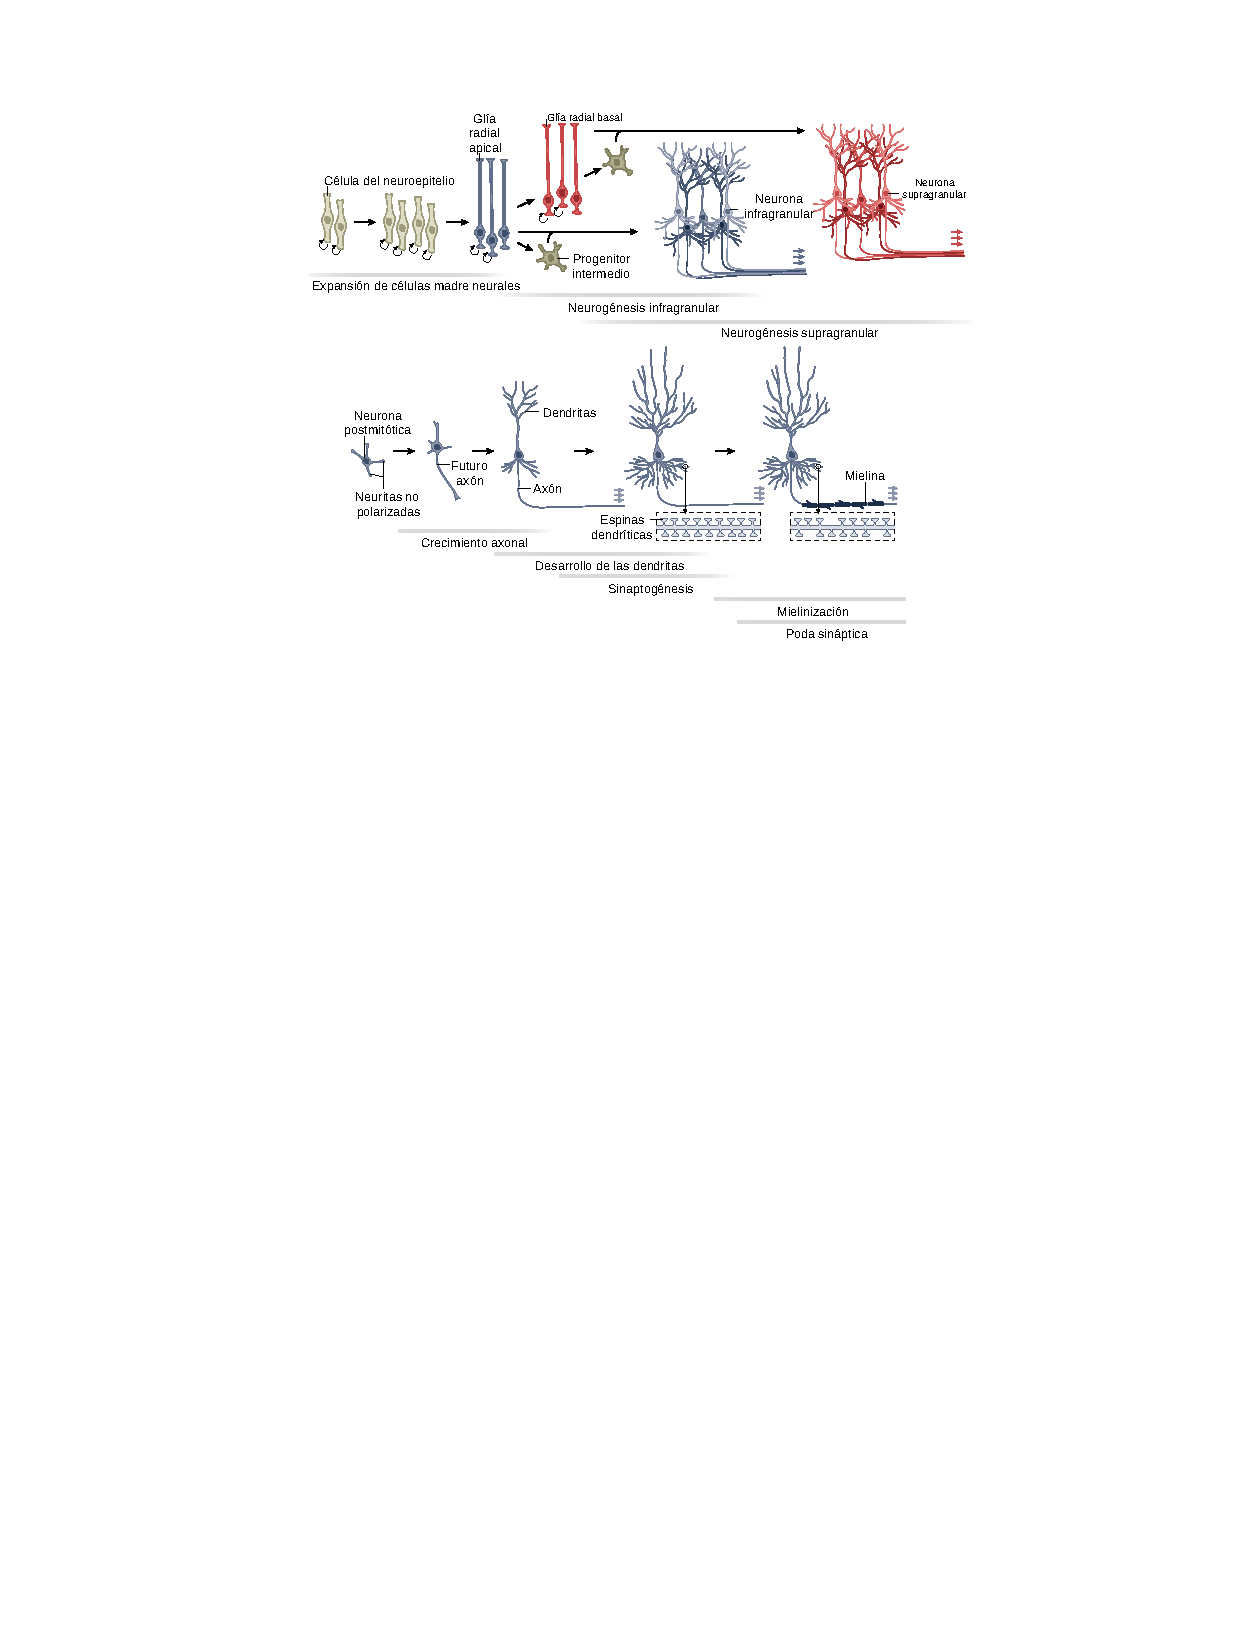
\includegraphics[width=1\textwidth]{embriologiacerebral}
	\captionsetup{font=footnotesize}
    \caption{Procesos biológicos del desarrollo cerebral. Modificado de:
	Lindhout FW, Krienen FM, Pollard KS y Lancaster MA. \cite{Lindhout2024}}
    \label{fig:embriologiacerebral}
\end{figure}

\subsubsection{Fase 6 - Muerte celular y poda sináptica}
La formación del cerebro también depende de procesos degenerativos que
comienzan en el período prenatal. La muerte celular programada o apoptosis se
inicia para reducir el número de células en el cerebro que no han logrado
establecer conexiones útiles o tienen conexiones infrautilizadas.
\cite{Gibb2018}

La muerte celular y la eliminación selectiva de procesos neuronales y sinapsis,
o poda en el desarrollo cerebral, son críticas para el comportamiento posnatal
normal. Típicamente, aproximadamente la mitad de las neuronas en la región
cortical mueren antes de la maduración final. Este proceso de muerte celular
programada, la apoptosis, se inicia y se mantiene por la expresión de genes
específicos. Un aspecto crítico en las fases finales de la secuencia hacia la
muerte celular es la activación de caspasas. \cite{Polin124}

La apoptosis parece ser desencadenada fundamentalmente por la competencia
neuronal por cantidades limitadas de factores tróficos, generados por el
objetivo, la entrada aferente o la glía asociada, permitiendo el emparejamiento
numérico de poblaciones neuronales interconectadas y la eliminación de
proyecciones aberrantes o incorrectas. \cite{Polin124}

\subsection{Desarrollo cerebral en el período postnatal}
Aunque la producción y migración de neuronas son principalmente eventos
prenatales, el desarrollo cerebral continúa de manera significativa después del
nacimiento. La proliferación y migración de progenitores gliales se extiende
durante un período prolongado después del nacimiento, mientras que la
diferenciación y maduración de estas células prosigue a lo largo de toda la
infancia. \cite{Stiles2010}

En el período postnatal, la neurogénesis continúa únicamente en un grado muy
limitado. No obstante, en la zona subventricular, nuevas neuronas siguen
emergiendo y migrando hacia el bulbo olfatorio. Asimismo, se producen neuronas
en el giro dentado del hipocampo, donde migran desde la capa subgranular
solamente hasta la cercana capa granular. Estas formas excepcionales de
neurogénesis parecen continuar durante toda la vida adulta, pero producen solo
un pequeño porcentaje de la población neuronal total.
\cite{Stiles2010}

En contraste con la neurogénesis limitada, la proliferación y migración de
progenitores gliales continúa durante un período prolongado mientras los
oligodendrocitos y astrocitos se diferencian. \cite{Stiles2010}

La sinaptogénesis que comenzó en el período prenatal continúa en el período
postnatal y a lo largo de toda la vida del individuo. La apoptosis continúa
desempeñando un papel fundamental en el desarrollo cerebral durante el período
postnatal. Las sinapsis poco utilizadas son eliminadas en un proceso denominado
poda sináptica, que optimiza los circuitos neuronales para mejorar la
eficiencia funcional. \cite{Gibb2018}

\subsubsection{Fase 7 - Mielinización}
Aunque cierta mielinización ocurre en el período prenatal, este proceso se
intensifica después del nacimiento y continúa hasta bien entrada la tercera
década de vida. El proceso de mielinización predice la maduración de áreas
corticales. Las áreas motoras y sensoriales primarias del cerebro se mielinizan
primero, mientras que las áreas de asociación lo hacen en último lugar.
\cite{Gibb2018}

En el tercer trimestre de gestación, los oligodendrocitos inmaduros desarrollan
extensiones lineales mientras envuelven los axones en preparación para la
mielinización. En el sistema nervioso central, los oligodendrocitos forman
hasta 40 segmentos separados de mielina en múltiples axones, a diferencia del
sistema nervioso periférico, donde las células de Schwann mielinizan axones
individuales. \cite{Polin124}

Los oligodendrocitos maduros se convierten en la etapa oligodendroglial
predominante en los meses posteriores al nacimiento a término y dan origen a la
mielinización. \cite{Polin124}

Después del inicio de la mielinización, los procesos intracelulares comienzan a
intensificarse para crear la composición rica en lípidos de la mielina. El
colesterol, los fosfolípidos y los glucoesfingolípidos representan el 70\% de
la membrana mielínica. Estas células han desarrollado un sistema altamente
eficaz para mantener la proporción óptima de clases de lípidos en la membrana
estrechamente envuelta para realizar su función aislante durante la conducción
nerviosa. \cite{Polin124}

\section{Modelo biopsicosocial del desarrollo infantil}
La biología influye en el comportamiento y el entorno, y a su vez, el
comportamiento y el entorno influyen en la biología a lo largo del desarrollo.
Los niños están influenciados directa e indirectamente tanto por su contexto
cercano como por factores sociales más amplios. El desarrollo infantil es el
producto de la acumulación de interacciones y experiencias cotidianas, así como
del contexto comunitario y cultural más amplio en el que se crían. Si bien los
eventos importantes (como cambios en la estructura familiar) y las
circunstancias (como los recursos familiares) son relevantes para el desarrollo
de los niños, también lo son las interacciones pequeñas que conforman la vida
cotidiana. \cite{Feldman3}

Las influencias tempranas, particularmente aquellas que producen niveles
tóxicos de estrés, afectan al individuo a través de su impacto en los sistemas
de respuesta al estrés del cuerpo, el desarrollo cerebral y la modificación de
la expresión genética. Los cambios epigenéticos, como la metilación del ADN y
la acetilación de histonas, pueden estar influenciados por experiencias
tempranas e impactar la expresión genética sin cambiar la secuencia de ADN.
Estos cambios pueden producir efectos duraderos en la salud y el bienestar del
individuo, y pueden transmitirse a generaciones futuras. \cite{Nelson19}

\subsection{Teorías principales}
Las influencias multinivel y transaccionales en el desarrollo infantil han sido
descritas en dos modelos teóricos fundamentales.

\subsubsection{Teoría de Sistemas Ecológicos de Bronfenbrenner}
La teoría de sistemas ecológicos de Urie Bronfenbrenner propone que existen
múltiples niveles de influencia en el desarrollo infantil, desde las relaciones
con los cuidadores hasta sistemas como las escuelas y lugares de trabajo, hasta
eventos en la sociedad más amplia. El microsistema describe las relaciones e
interacciones directas que tienen los niños, como con cuidadores, hermanos y
compañeros. Estas personas influyen directamente en el niño proporcionando
oportunidades para jugar y aprender, y brindando apoyo emocional. El
microsistema también contiene estructuras con las que el niño interactúa, como
la escuela, el vecindario, entornos de cuidado infantil y la familia. Los niños
tanto influyen como son influenciados por estas relaciones y estructuras.
\cite{Feldman3}

\begin{wrapfigure}{r}[-0.65cm]{0.40\textwidth}
	\centering
    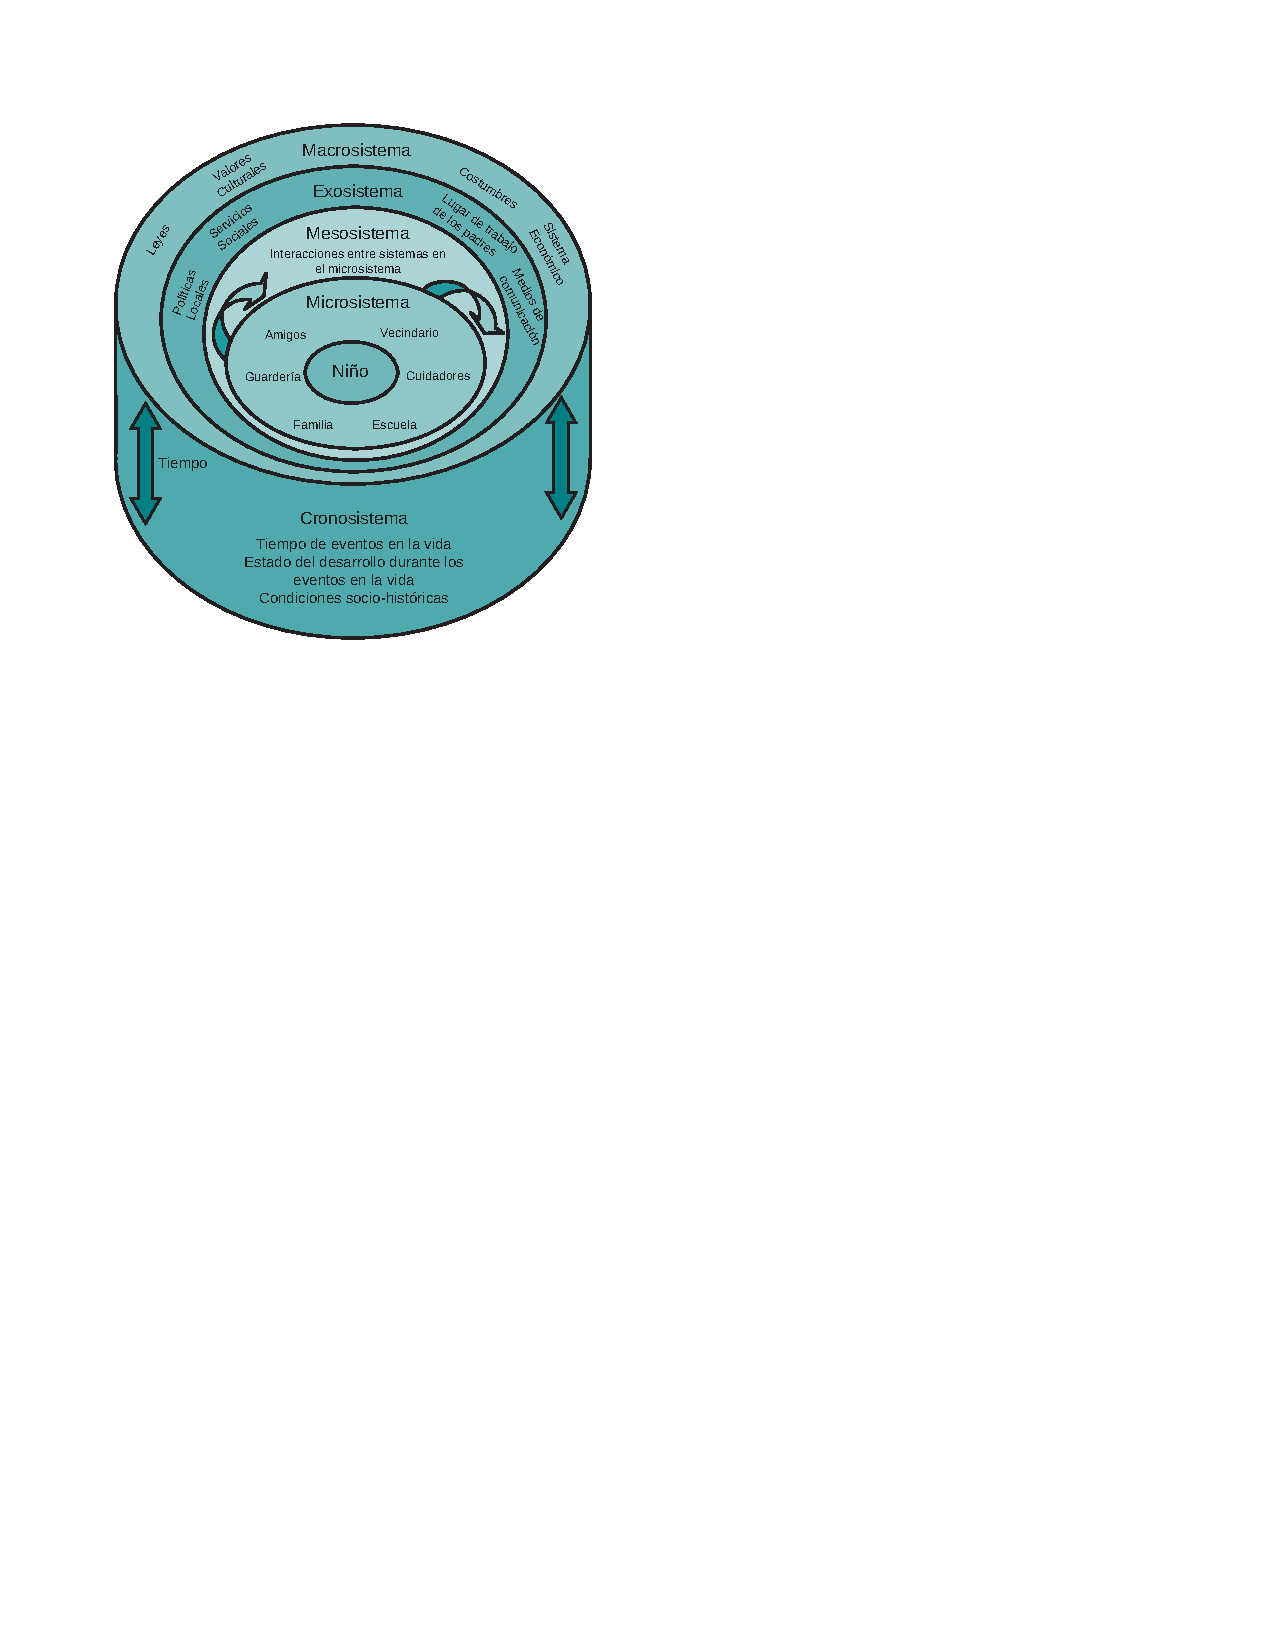
\includegraphics[width=1\linewidth]{sistemasbronfenbrenner}
	\captionsetup{font=footnotesize}
    \caption{La teoría de Bronfenbrenner describe los múltiples niveles que
    impactan al niño en un momento dado y durante el curso del desarrollo.
    Modificado de: Julian M y Lumeng J. \cite{Feldman3}}
    \label{fig:sistemasbronfenbrenner}
\end{wrapfigure}

El mesosistema describe la interacción entre las estructuras que están en el
microsistema. El exosistema consiste en sistemas sociales más grandes que
impactan estructuras en el microsistema. Los niños no interactúan directamente
con el exosistema, pero experimentan el impacto de los cambios en estos sistemas
sociales. El macrosistema es la capa más externa del entorno de un niño y está
definido por valores culturales, costumbres y leyes que influyen en el
funcionamiento de las capas internas. El cronosistema captura la influencia del
tiempo en el desarrollo infantil, reflejando tanto los procesos de desarrollo
que tienen lugar a lo largo del tiempo como la influencia cambiante de los
eventos según su duración y la etapa de desarrollo en la que ocurren.
\cite{Feldman3}

Comprender el ecosistema más amplio del niño es crucial para entender su 
entorno familiar y el contexto de su desarrollo. Factores como la pobreza, el 
racismo, el acceso a la educación, el transporte, los alimentos, la vivienda,
el empleo de los padres y los sistemas de apoyo local influyen
significativamente en el bienestar de un niño. Siempre que sea posible, 
identificar los recursos y activos comunitarios para las familias puede ayudar 
a promover la salud y el desarrollo. \cite{Nelson19}

\subsubsection{Modelo Transaccional de Sameroff}
El modelo transaccional de Arnold Sameroff se basa en las ideas de
Bronfenbrenner sobre la bidireccionalidad de los efectos en el desarrollo
infantil. Discute los procesos que tienen lugar entre padres e hijos en las
interacciones cotidianas y a lo largo del tiempo. Los entornos de los niños
moderan el efecto de los riesgos biológicos tempranos en su desarrollo. La
naturaleza y la crianza se consideran inherentemente inseparables; los genes se
expresan dependiendo del entorno, y los padres responden de manera diferente a
los niños según las características biológicas inherentes del niño.
\cite{Feldman3}

Las características de un niño impactan la crianza, y la crianza impacta el
desarrollo infantil; estas cascadas bidireccionales de influencias continúan a
lo largo del tiempo durante el desarrollo. Es fundamental entender que los
comportamientos de los padres en respuesta a los niños están impulsados por
sus interpretaciones y el significado que extraen del comportamiento. Por
ejemplo, el manejo ansioso de un padre puede surgir debido a su percepción
sobre las complicaciones del nacimiento del niño; un padre puede desvincularse
de un niño con un temperamento difícil debido al significado que atribuye al
comportamiento inquieto del niño. \cite{Sameroff2009}

\subsubsection{Modelo de Diátesis-Estrés}
Este modelo sugiere que algunos individuos son más vulnerables a los impactos
del estrés que otros. Las diátesis o predisposiciones hereditarias o
constitucionales pueden incluir factores biológicos, genéticos, relacionados
con el temperamento o cognitivos que predisponen a un niño a ser vulnerable a
las influencias del estrés. En un entorno favorable para el desarrollo, este
modelo sugiere que tanto los individuos resilientes como los vulnerables
probablemente se desarrollarán bien. En un entorno desafiante, los individuos
resilientes se desarrollarían bien, mientras que los vulnerables no.
\cite{Feldman3}

\subsubsection{Teoría de Susceptibilidad Diferencial}
Esta teoría postula que los individuos varían en su plasticidad, o su nivel de
susceptibilidad a las influencias ambientales. \cite{Belsky2021} Algunos niños,
a veces denominados ``orquídeas'', son muy sensibles a su entorno. Cuando están
en un entorno que apoya ampliamente su desarrollo y bienestar, prosperan; sin
embargo, cuando están en un entorno que no apoya su desarrollo, tienen
dificultades. Otros niños, a veces denominados ``dientes de león'', son menos
susceptibles a las influencias ambientales y se desarrollarán más o menos de la
misma manera independientemente de cuán favorable sea su entorno y sus
relaciones. Los niños pueden ubicarse en cualquier punto del espectro entre
estos dos extremos. \cite{Belsky2021}

\subsection{Relaciones cuidador-niño}
Los cuidadores impactan la biología de un niño a través de sus interacciones con
él. Las interacciones que un niño tiene con el cuidador, o respaldadas por él,
dejan una marca duradera en el genoma del niño y en la estructura cerebral.
A través de la poda neuronal, las conexiones neuronales del niño se refuerzan o
se eliminan según sus experiencias. Los efectos epigenéticos, incluidos los
relacionados con la experiencia del cuidado temprano, también están activos
durante este período de desarrollo. \cite{Roth2011}

La influencia del entorno de crianza domina la mayoría de los modelos actuales
de desarrollo. Los bebés en hospitales y orfanatos, carentes de oportunidades
para el apego, tienen déficits de desarrollo severos. El apego se refiere a
una tendencia determinada biológicamente de un niño pequeño a buscar
proximidad con sus padres durante momentos de estrés y a la relación que
permite a los niños con apego seguro utilizar a sus padres para restablecer una
sensación de bienestar después de una experiencia estresante. El apego inseguro
puede ser predictivo de problemas de comportamiento y aprendizaje posteriores.
\cite{Nelson19}

En todas las etapas del desarrollo, los niños progresan de manera óptima
cuando tienen cuidadores adultos que prestan atención a sus señales verbales y
no verbales y responden en consecuencia. En la primera infancia, esta
capacidad de respuesta contingente a signos de sobreestimulación o baja
estimulación ayuda a mantener a los infantes en un estado de alerta tranquila y
fomenta la autorregulación autonómica. Las respuestas contingentes consistentes
(refuerzo dependiente del comportamiento del otro) a gestos no verbales crean
la base para la atención compartida y la reciprocidad que son críticas para el
desarrollo posterior del lenguaje y social. \cite{Nelson19}

Los cuidadores sirven como guía para el desarrollo cognitivo, social,
conductual, emocional y físico de los infantes. La crianza sensible y receptiva
promueve resultados positivos en los niños en dominios que incluyen el apego,
el desarrollo cognitivo, las habilidades sociales y la regulación emocional.
Un cuidador sensible y receptivo está sintonizado con los sentimientos y
necesidades del niño, y responde con prontitud con acciones que están en
sintonía con los sentimientos y necesidades del niño durante las
actividades cotidianas. \cite{Feldman3}

\subsection{Estrés y trauma infantil}
Incluso a edades tempranas, muchos niños están expuestos a niveles de estrés y
trauma que pueden impactar su desarrollo. El estrés positivo se considera una
parte normal del desarrollo saludable. Las relaciones de cuidado son clave para
amortiguar el efecto de estos factores estresantes, haciendo que los factores
estresantes sean más manejables y que las respuestas biológicas al estrés
disminuyan. El estrés tóxico implica elevaciones del sistema de estrés fuertes,
frecuentes y prolongadas que pueden causar cambios duraderos en los sistemas
neurobiológicos, teniendo un efecto perjudicial en la salud física y mental
posterior. \cite{Feldman3}

Los niños que han experimentado trauma comúnmente presentan comportamiento
agresivo, irritabilidad y retraimiento emocional. Muchos niños volverán a
escenificar el trauma que han experimentado o presenciado, ya sea en vivo o a
través del juego. A menudo, estos factores estresantes ocurren en el contexto
de relaciones de cuidado (ej. abuso o negligencia infantil), lo que magnifica la
experiencia sentida de estrés y disminuye el potencial de amortiguación del
estrés a través de las relaciones. Cuando ocurren en el contexto de relaciones
socioemocionales de apoyo, detección temprana e intervención efectiva, es
probable que estos factores estresantes sean tolerables. \cite{Feldman3}

Los determinantes sociales de la salud son contribuyentes clave a los factores
estresantes y traumas que podrían conducir a elevaciones crónicas en los
sistemas de respuesta al estrés biológico e impactar el desarrollo de los
niños. Las familias que experimentan racismo, discriminación u opresión
económica a menudo experimentan elevaciones crónicas en sus sistemas de
respuesta al estrés biológico que pueden contribuir a una sensación
generalizada de falta de seguridad y protección. Los padres que están
experimentando estos factores estresantes comprensiblemente pueden tener menos
capacidad psicológica para apoyar a sus hijos, ya que es exponencialmente más
difícil ayudar a un niño a sentirse seguro y protegido. \cite{Feldman3}

\section{Teorías del desarrollo y la cognición}
\subsection{Teorías cognitivas}
El desarrollo cognitivo se comprende mejor a través del trabajo de Piaget. Un
principio central del trabajo de Piaget es que la cognición cambia en calidad,
no solo en cantidad. Piaget describió cómo los niños construyen activamente
conocimiento por sí mismos a través de los procesos vinculados de asimilación
(incorporar nuevas experiencias según esquemas existentes) y acomodación (crear
nuevos patrones de comprensión para adaptarse a nueva información). De esta
manera, los niños están continuamente reorganizando activamente los procesos
cognitivos. \cite{Nelson19}

\subsubsection{Jean Piaget: Desarrollo cognitivo}
Jean Piaget (1896-1980) centró su teoría del desarrollo en cómo el niño
desarrolla un marco lógico y científico para comprender el mundo físico.
Postuló que la comprensión de los niños pasa por una serie de cambios
cualitativos o etapas vinculadas a la edad. Cada etapa es un filtro que
selecciona y organiza lo que el niño percibe y entiende. Cada etapa es un marco
que proporciona los componentes básicos para la siguiente, por lo que hay un
orden definido en el que surge la comprensión. El desarrollo ocurre cuando los
niños descubren una discrepancia entre su comprensión actual de la realidad
(asimilación) y las características del mundo que no encajan con esa
comprensión (acomodación). \cite{Feldman3}

Piaget propuso la teoría más conocida del desarrollo cognitivo. En esta teoría,
el desarrollo cognitivo se despliega en cuatro etapas desde la infancia hasta
la adolescencia. Piaget veía el desarrollo cognitivo como una propiedad
inherente a la biología humana, y por lo tanto consideraba las etapas
universales. La suya es una visión constructivista en la que el conocimiento se
desarrolla a través de las actividades de los niños y sus esfuerzos por dar
sentido a sus experiencias. Debido a que el momento de la experiencia puede
variar entre los niños, Piaget asignó edades aproximadas para las etapas.
\cite{Gauvain2022}

Piaget describió dos procesos que regulan el desarrollo cognitivo: organización
y adaptación. La organización se refiere a la estructura secuencial del
desarrollo mental desde un sistema simple a uno más complejo. La adaptación
pertenece a cómo el conocimiento en desarrollo coincide con el entorno, e
incluye dos funciones complementarias. En la asimilación, se añade nueva
información al conocimiento existente, y en la acomodación, se modifica el
conocimiento existente para incluir nueva información. El propósito de la
adaptación es mejorar la alineación entre el pensamiento del individuo y el
entorno, lo que Piaget llamó equilibración. \cite{Gauvain2022}

Con el desarrollo, el pensamiento de los niños cambia desde un enfoque en
experiencias sensoriales y motoras inmediatas y formas simples de entender e
interactuar con el mundo hacia formas más complejas y abstractas de pensar. Las
cuatro etapas que se centran principalmente en el razonamiento lógico; son el
período sensoriomotor (0-2 años), preoperacional (2-6 años), operaciones
concretas (6-11 años) y operaciones formales (más de 11 años), estas etapas se
resumen en el cuadro \ref{tab:piaget-stages}.
\cite{Gauvain2022}

\begin{table}[htbp]
\caption{Características de las etapas principales en la teoría de Piaget}
\label{tab:piaget-stages}
\fontsize{9}{9}\selectfont
\begin{tabular}{ll}
\hline
Etapa y rango de edad aproximado & Características principales \\ \hline
Sensoriomotor: nacimiento a 2 años & \begin{tabular}[c]{@{}l@{}}La inteligencia está limitada a las propias acciones del infante sobre el\\entorno. La cognición progresa desde el ejercicio de reflejos\\(por ejemplo, succión, orientación visual) hasta el inicio del\\funcionamiento simbólico.\end{tabular} \\
Preoperacional: 2 a 7 años & \begin{tabular}[c]{@{}l@{}}La inteligencia es simbólica, expresada a través del lenguaje, imágenes,\\y otros modos, permitiendo a los niños representar mentalmente y\\comparar objetos fuera de la percepción inmediata. El pensamiento\\es intuitivo en lugar de lógico y es egocéntrico, en el sentido de que\\los niños tienen dificultad para adoptar la perspectiva de otro.\end{tabular} \\
Operaciones concretas: 7 a 11 años & \begin{tabular}[c]{@{}l@{}}La inteligencia es simbólica y lógica, el pensamiento es menos\\egocéntrico. El pensamiento de los niños está limitado a fenómenos\\concretos y sus propias experiencias pasadas; es decir, el pensamiento\\no es abstracto.\end{tabular} \\
Operaciones formales: 11 a 16 años & \begin{tabular}[c]{@{}l@{}}Los niños son capaces de formular y probar hipótesis; la posibilidad\\domina la realidad. Los niños son capaces de reflexionar sobre sus\\propios procesos de pensamiento y, generalmente, pueden pensar\\de manera abstracta.\end{tabular} \\ \hline \hline
\footnotesize Modificado de: Bjorklund \cite{Bjorklund2011-aa}
\end{tabular}
\end{table}

\subsection{Teorías socioculturales}
\subsubsection{Lev Vygotsky: Influencias ambientales en el lenguaje y el pensamiento}
Al igual que Piaget, Lev Vygotsky (1896-1934) estaba interesado en el origen
del conocimiento y de las habilidades de razonamiento, y como Bowlby, estaba
interesado en los efectos de las relaciones humanas en el desarrollo. Desde la
perspectiva de Vygotsky, todos los aspectos del desarrollo humano son el
resultado de interacciones con personas con más experiencia. Esas interacciones
reflejan prácticas culturales. En algunas culturas, se dirige muy poco discurso
hacia los niños pequeños, mientras que en otras culturas se espera que los
niños participen en una conversación. \cite{Feldman3}

El aprendizaje a través de la interacción con otros con mayor experiencia
comienza en la infancia y continúa a lo largo del desarrollo. El otro más
experimentado ayuda a un niño a construir recuerdos, resolver un problema, notar
aspectos del entorno o elaborar sobre la comunicación verbal. \cite{Feldman3}

Otro enfoque importante de la teoría de Vygotsky se refiere al papel del
lenguaje en la formación del pensamiento del niño. Mientras que el pensamiento
y el lenguaje emergen como habilidades humanas independientes, el lenguaje, que
expresa pensamientos, llega a regular primero a través de su expresión externa,
pero más tarde a través de su internalización y expresión en la mente del niño.
\cite{Feldman3}

\subsubsection{Reuven Feuerstein: Mediación social de la cognición}
La teoría y el trabajo aplicado de Reuven Feuerstein (1921-2014) se centran en
la maleabilidad de la cognición e inteligencia de los niños en cada etapa del
desarrollo. Feuerstein teorizó que el desarrollo cognitivo es producto de dos
modalidades de interacción entre el organismo y el entorno. \cite{Feldman3}

Feuerstein distingue entre dos grupos de determinantes del desarrollo cognitivo
diferencial. El primer grupo de determinantes incluye factores genéticos, el
nivel de estimulación ambiental, las relaciones emocionales entre el niño y los
mediadores, y el estatus socioeconómico. En condiciones desfavorables, estos
determinantes interfieren con el desarrollo cognitivo. El segundo grupo de
determinantes consiste en la falta o reducción de exposición a la experiencia
de aprendizaje mediado. \cite{Feldman3}

\subsubsection{Urie Bronfenbrenner: Influencias ambientales directas e indirectas}
Urie Bronfenbrenner (1917-2005) amplió la descripción del entorno que el niño
en crecimiento experimenta tanto directa como indirectamente. Postuló cinco
niveles de influencias ambientales. El más inmediato es el microsistema, que
consiste en entornos sociales que el niño experimenta directamente, como la
familia, los compañeros y la escuela. El microsistema está incrustado en el
mesosistema, el sistema interconectado de microsistemas en los que participa
una persona. El siguiente nivel es el exosistema, que incluye vecinos, medios
sociales y de masas, servicios sociales, industria y política local. Estos
influyen en las personas que influyen en el niño. Más allá está el
macrosistema, las actitudes y creencias de la cultura. Todos estos sistemas
están incrustados en un contexto histórico llamado cronosistema. Estos niveles
del entorno forman una red de conexiones, y el individuo está en su centro
potencialmente influyendo en los niños mientras buscan activamente adaptarse a
su mundo. \cite{Feldman3}

\subsection{Teoría de sistemas dinámicos}
Uno de los enfoques más nuevos para el desarrollo es la teoría de sistemas
dinámicos. Los procesos que pueden explicar el cambio de comportamiento (ej.
potencial genético, procesos neurológicos, características físicas,
estructura familiar, metas y motivos personales) están entrelazados, no son
factores causales independientes. El desarrollo es el resultado de la
interacción de procesos en muchos niveles y muchos sistemas. El desarrollo es
moldeado por fuerzas dentro y fuera de la persona, fusionándose e influyéndose
mutuamente para producir nuevas capacidades y comportamientos. \cite{Newman2020}

El núcleo de la teoría descansa en la definición de sistemas. Todos los
sistemas (biológicos y sociales) están compuestos por elementos
interdependientes que comparten funciones, límites, metas e identidad
interrelacionados. Un sistema dinámico cambia continuamente para llevar a cabo
sus funciones de una manera que mantiene la interacción fluida entre sus
componentes, preservando así el equilibrio. Los elementos se influyen entre sí
y se cambian unos a otros con el tiempo. Entender el desarrollo requiere
considerar eventos momento a momento y su interacción con características
individuales cambiantes. Requiere trazar un camino desde un punto en el tiempo
hasta un punto posterior cuando emerge un comportamiento nuevo y más maduro.
Esto requiere un análisis detallado de múltiples aspectos del comportamiento y
una investigación del proceso de reorganización y crecimiento. La teoría ayuda
a especificar las propiedades de los sistemas que están en flujo (sistemas
abiertos) y cómo la retroalimentación actúa para regular el cambio.
\cite{Feldman3}

La palabra dinámico se utiliza para resaltar la interacción constante y la
influencia mutua de los elementos del sistema. Un componente clave es la
autoorganización, la idea de que el desarrollo se produce a través de las
interacciones de los diversos elementos del sistema. Juntos, estos elementos
producen un conjunto de comportamientos que conducen al cambio cognitivo.
\cite{Gauvain2022}

\section{Trastornos del neurodesarrollo y factores de riesgo}
De acuerdo con el Manual Diagnóstico y Estadístico de los Trastornos Mentales
\cite{DSM5TR}, los trastornos del neurodesarrollo constituyen un grupo de 
afecciones que se manifiestan en las etapas tempranas del desarrollo, 
frecuentemente antes de que el niño ingrese a la escuela, y se caracterizan 
por déficits que producen limitaciones en áreas específicas o globales del
funcionamiento personal, social y académico.

Los trastornos del neurodesarrollo frecuentemente coexisten entre sí; por 
ejemplo, los niños con trastorno del espectro autista a menudo presentan 
trastorno del desarrollo intelectual, y muchos niños con trastorno por déficit
de atención e hiperactividad también presentan algún trastorno específico del
aprendizaje. \cite{DSM5TR}

El DSM-5-TR clasifica los trastornos del neurodesarrollo en seis categorías:
    \begin{itemize}
        \item Trastorno del desarrollo Intelectual
        \item Trastornos de la comunicación
        \item Trastorno del espectro autista
        \item Trastorno por déficit de atención e hiperactividad
        \item Trastorno específico del aprendizaje
        \item Trastornos motores
    \end{itemize}

\subsection{Trastorno del desarrollo intelectual}
\subsubsection{Definición}
El trastorno del desarrollo intelectual se caracteriza por limitaciones 
significativas tanto en el funcionamiento intelectual como en la conducta 
adaptativa, que se manifiestan antes de los 18 años y se expresan en 
habilidades adaptativas conceptuales, sociales y prácticas. \cite{Simms2023}

El funcionamiento adaptativo incluye tres amplios dominios: conceptual, social
y práctico. El dominio conceptual involucra la competencia académica, la
adquisición de conocimientos prácticos y el juicio en situaciones nuevas. El
dominio social implica la conciencia de los pensamientos y sentimientos de los
demás, la empatía, las amistades y el juicio social. El dominio práctico abarca
la capacidad para gestionar los asuntos propios, incluyendo las
responsabilidades escolares y laborales, el manejo del dinero y las
actividades recreativas. \cite{Simms2023}

\subsubsection{Epidemiología}
La prevalencia mundial del trastorno del desarrollo intelectual se estima
entre el 1\% y el 3\%. Se estima que la prevalencia es aproximadamente de 16.4
por cada 1,000 personas en países de bajos ingresos, alrededor de 15.9 por cada
1,000 en países de ingresos medios, y aproximadamente 9.2 por cada 1,000 en
países de altos ingresos. \cite{vanKarnebeek2018, Nelson56}

\subsubsection{Factores de riesgo}
Numerosas causas identificadas del trastorno del desarrollo intelectual pueden
ocurrir antes del nacimiento, durante el parto, después del nacimiento o más 
tarde en la infancia. Estas incluyen infecciones, traumatismos, prematuridad,
hipoxia-isquemia, exposiciones a tóxicos, disfunción metabólica, anomalías
endocrinas, desnutrición y anomalías genéticas \cite{Nelson56}.

Las formas leves y más graves del trastorno presentan factores de riesgo y
etiologías diferentes pero que se sobreponen. Los factores de riesgo no
genéticos frecuentemente asociados con formas leves incluyen bajo nivel
socioeconómico, bajos niveles de educación materna, residencia en un país en
desarrollo, desnutrición y acceso limitado a la atención sanitaria. Las causas
biológicas más comunes o factores de riesgo para las formas leves incluyen
restricción del crecimiento intrauterino, prematuridad, insultos perinatales,
exposición intrauterina a drogas, exposición postnatal a sustancias
neurotóxicas (como el plomo), algunas anomalías cromosómicas sexuales y algunos
síndromes genéticos con múltiples anomalías congénitas mayores o menores
\cite{Nelson56}.

En niños con formas más graves del trastorno, se puede identificar una causa
biológica en aproximadamente tres cuartas partes de los casos. Las causas
incluyen trastornos cromosómicos (ej. síndrome de Down, Wolf-Hirschhorn y
deleción 1p36) y otros trastornos genéticos y epigenéticos (ej. síndromes de X
frágil, Rett y Angelman), anomalías del desarrollo cerebral, errores innatos del
metabolismo y trastornos mitocondriales \cite{Nelson56}.

\subsubsection{Diagnóstico}
El diagnóstico formal del trastorno del desarrollo intelectual requiere la
evaluación con pruebas individuales de inteligencia y funcionamiento
adaptativo.

La Escala Bayley de Desarrollo Infantil es la prueba de inteligencia infantil
más utilizada, proporciona una evaluación de las capacidades cognitivas, del
lenguaje, motoras, conductuales, socioemocionales y adaptativas generales para
niños desde los 16 días a los 42 meses de edad. \cite{Nelson56}

Las pruebas de inteligencia más utilizadas para niños mayores de 3 años son las
Escalas Wechsler. Para niños con marcadas limitaciones del lenguaje o verbales,
se pueden emplear pruebas como las Escalas de Habilidades Diferenciales-II o la
Escala Internacional de Rendimiento Leiter, para captar de manera óptima las
habilidades de rendimiento no verbal. \cite{Nelson56}

\subsection{Trastornos de la comunicación}
Los trastornos de la comunicación incluyen déficits en el lenguaje, el habla y
la comunicación. El habla es la producción expresiva de sonidos e incluye la
articulación, fluidez, voz y resonancia de un individuo. El lenguaje abarca la
forma, función y uso de un sistema convencional de símbolos gobernado por reglas
para la comunicación. La comunicación incluye cualquier comportamiento verbal o
no verbal que influye en las ideas, actitudes o comportamientos de otro
individuo. \cite{DSM5TR}

\subsubsection{Trastorno del lenguaje}
Las características esenciales del trastorno del lenguaje son las dificultades
en la adquisición y uso del lenguaje debido a déficits en la comprensión o
producción de vocabulario, gramática, estructura de las oraciones y discurso.
Los déficits del lenguaje son evidentes en la comunicación hablada, escrita o
mediante lenguaje de señas. \cite{DSM5TR}

Los trastornos primarios del desarrollo del habla y lenguaje son dificultades
significativas que se encuentran en ausencia de disfunción cognitiva, sensorial
o motora importante. El criterio para el retraso del lenguaje es un rendimiento
de al menos 1.5 a 2 desviaciones estándar por debajo de la media poblacional en
pruebas estandarizadas de habla o lenguaje. \cite{Feldman44}

Los niños con trastorno del lenguaje pueden tener dificultades significativas
en habilidades lingüísticas de nivel superior, habilidades de razonamiento, la
capacidad para adoptar la perspectiva de otra persona, y la habilidad para
parafrasear y reformular. Algunos niños con este trastorno muestran dificultades
en la interacción social, ya que las interacciones sociales a menudo están
mediadas por el lenguaje verbal. \cite{Nelson53}

\paragraph{Epidemiología}
Los trastornos del lenguaje y del habla son altamente prevalentes.
Aproximadamente el 16\% de los niños muestran retrasos clínicamente
significativos a los 2 años; cerca de la mitad de estos niños continúan
con retrasos hasta el inicio de preprimaria. Los trastornos del lenguaje y habla
pueden ocurrir de forma aislada, juntos o en conjunción con otros retrasos o
trastornos. \cite{Feldman44}

\paragraph{Factores de riesgo}
Los factores genéticos parecen desempeñar un papel importante en cómo los niños
aprenden a hablar. Los antecedentes familiares pueden identificar problemas de
habla o lenguaje actuales o pasados en hasta el 30\% de los familiares de
primer grado de niños afectados. La tasa de concordancia para puntuaciones
bajas en pruebas de lenguaje o antecedentes de terapia del habla dentro de
pares de gemelos es aproximadamente del 50\% en pares dicigóticos y del 90\%
en pares monocigóticos. Factores ambientales, hormonales y nutricionales pueden
ejercer influencias epigenéticas al desregular la expresión génica.
\cite{Nelson53}

Los niños criados en orfanatos típicamente experimentan trastornos del
lenguaje y del habla. Los niños que han sufrido abuso y negligencia también
desarrollan frecuentemente trastornos del lenguaje. Para niños que viven en
pobreza, los retrasos en el lenguaje pueden estar relacionados con una pobre
nutrición lingüística y otros desafíos, como mala nutrición y altos niveles
de estrés. \cite{Feldman44}

\paragraph{Diagnóstico}
La evaluación precisa de bebés y niños pequeños es desafiante debido a la
baja frecuencia de producción verbal y la dificultad que tienen los niños
pequeños para cooperar con los clínicos. Las observaciones informales, las
herramientas de entrevista con los padres y las evaluaciones naturales juegan
un papel importante en la evaluación de los niños pequeños. Las evaluaciones
formales se vuelven más relevantes a medida que el niño alcanza la edad
preescolar. \cite{Nelson53}

\paragraph{Comorbilidades}
El trastorno del lenguaje puede asociarse con otros trastornos del
neurodesarrollo en términos de trastorno específico del aprendizaje
(alfabetización y aritmética), trastorno del desarrollo intelectual, trastorno
por déficit de atención e hiperactividad, trastorno del espectro autista y
trastorno de la coordinación del desarrollo. \cite{Feldman44}

\subsubsection{Trastornos de los sonidos del habla}
Un trastorno de los sonidos del habla representa una alteración en la
capacidad para producir los sonidos de las palabras del lenguaje. Un síntoma
primario de la alteración del habla puede ser un discurso ininteligible. Los
trastornos del habla se describen en términos de las características de los
errores de los sonidos del habla o la causa del problema. A menudo no se puede
identificar una causa subyacente para el trastorno de los sonidos del habla.
\cite{Feldman44}

\paragraph{Trastornos de articulación}
La incapacidad para producir correctamente los sonidos del habla se conoce
como trastorno de articulación. Los niños con trastornos de articulación
típicamente muestran errores en un pequeño subconjunto de sonidos
(p. ej., /r, l, s/). En la mayoría de los casos, la causa de un trastorno de
articulación es desconocida; se presume que son resultado de un aprendizaje
incorrecto. Una causa conocida de trastornos de articulación es la pérdida
auditiva bilateral leve a moderada permanente. \cite{Feldman44}

\paragraph{Trastornos fonológicos}
Cuando un niño muestra errores de habla basados en patrones o reglas
implícitas a pesar de la capacidad para producir los mismos sonidos
correctamente en otros contextos, la condición se denomina trastorno
fonológico. Un niño que omite las consonantes finales puede decir ``feli'' en
lugar de ``feliz'' y ``canta'' en lugar de ``cantar'', pero probablemente no
tenga ningún problema al decir palabras como ``zombi'' o ``rana''. El niño está
aplicando una regla incorrecta en lugar de mostrar una incapacidad para
producir el sonido correctamente. \cite{Feldman44}

Los niños con errores fonológicos típicamente tienen déficits moderados a
graves en las habilidades del habla.

\paragraph{Trastornos anatómicos}
La anquiloglosia, o frenillo lingual corto, es una anomalía congénita común
que se ha supuesto que afecta al habla. Sin embargo, la anquiloglosia
típicamente no causa alteraciones del habla. Aunque el frenillo lingual puede
ser significativo al nacer, su gravedad disminuye con el tiempo a medida que
las estructuras orales crecen. Además, los sonidos del habla pueden producirse
con una elevación mínima de la lengua. Cortar el frenillo lingual
típicamente no mejora el habla. Una excepción pueden ser los niños con
parálisis cerebral cuya anquiloglosia está relacionada con alteraciones
neurológicas. \cite{Feldman44}

Los niños con paladar hendido tienen un alto riesgo de presentar trastornos
fonológicos y déficits del lenguaje. Incluso después de la reparación de un
paladar hendido aislado, pueden exhibir patrones de articulación inusuales o
idiosincrásicos. Las estructuras velofaríngeas funcionan anormalmente,
resultando en una incapacidad para generar suficiente presión de aire
intraoral para la producción de consonantes. \cite{Feldman44}

Algunos niños tienen insuficiencia velofaríngea aislada por razones
desconocidas. Estos niños están en riesgo de presentar trastornos de los
sonidos del habla similares a los de los niños con paladar hendido.
\cite{Feldman44}

\paragraph{Trastornos neurológicos}
La disartria es un trastorno del habla asociado con trastornos neuromotores,
como la parálisis cerebral. El tono muscular elevado, la pobre coordinación de
los movimientos motores y la deficiente coordinación de la respiración y la
producción de sonido resultan en movimientos musculares lentos y limitado rango
de movimiento. El habla disártrica tiene una calidad arrastrada y forzada, que
afecta la precisión de la producción de sonidos del habla, la velocidad, el
tono y la entonación. \cite{Feldman44}

La apraxia del habla infantil, conocida anteriormente como apraxia verbal del
desarrollo o dispraxia, es una condición en la que los niños tienen
dificultad con la producción controlada de los sonidos del habla. La etiología
presunta es de origen neurológico, aunque generalmente no se encuentran
lesiones anatómicas. Los niños cometen errores en la producción de vocales y
consonantes y muestran una enorme variabilidad en cómo producen los fonemas y
en el volumen. La inconsistencia en la producción y en los errores hace que la
interpretación de su habla sea muy desafiante. \cite{Feldman44}

\paragraph{Tartamudeo}
El tartamudeo es la causa más común de disfluencia significativa, manifestada
por repetición de sonidos y sílabas y prolongación de vocales o consonantes
realizadas con un flujo de aire continuo. El tartamudeo a menudo se acompaña
de pausas inapropiadas, expresiones faciales repetitivas u otras rutinas
conductuales. Actualmente se considera un trastorno del neurodesarrollo,
caracterizado por el desarrollo atípico de redes neuronales involucradas en la
planificación y ejecución motora del habla. El tartamudeo tiene agregación
familiar, lo que sugiere contribuciones genéticas. \cite{Feldman44}

\subsection{Trastorno del espectro autista}
El trastorno del espectro autista (TEA) representa un grupo de trastornos del
neurodesarrollo que aparecen durante la primera infancia y se caracterizan por
una alteración en la comunicación e interacción social, acompañada de
comportamientos restrictivos y repetitivos.

\subsubsection{Definición del trastorno del espectro autista}
La primera descripción clínica de seis niños con una constelación de rasgos
fácilmente reconocibles como lo que actualmente se conoce como TEA fue
publicada por la psiquiatra rusa Grunya Sukhareva en 1925. \cite{Myers2025}

En 1943, Leo Kanner describió elocuentemente a 11 niños con ``alteraciones
autistas innatas del contacto afectivo'' caracterizadas por un compromiso
social y de interacción profundamente deficiente; alteraciones en la
comunicación que variaban desde el mutismo hasta la ecolalia, inversión
pronominal y literalidad; e interacciones inusuales con el entorno, incluyendo
un ``deseo obsesivo y ansioso por el mantenimiento de la igualdad'' que no se
explicaba por un deterioro cognitivo general. \cite{Myers2025}

Antes del DSM-5, cinco trastornos superpuestos capturaban el espectro:
trastorno autista, trastorno de Asperger, trastorno desintegrativo infantil,
síndrome de Rett y trastorno generalizado del desarrollo no especificado.
\cite{Boland2021-by}

El DSM-5 y la CIE-11 están bien alineados en su conceptualización del TEA como
un diagnóstico único definido por déficits clínicamente significativos y
persistentes en la comunicación e interacción social y comportamientos e
intereses restrictivos y repetitivos atípicos que causan un deterioro
significativo en el funcionamiento adaptativo. Las manifestaciones específicas
de los déficits centrales varían con la edad, la capacidad lingüística e
intelectual, y la gravedad del trastorno. Los síntomas comienzan en el período
de desarrollo, pero pueden no manifestarse completamente hasta que las demandas
sociales excedan las capacidades limitadas. Los déficits en la comunicación e
interacción social deben estar presentes en un grado fuera del rango esperado
de funcionamiento para la edad y el nivel de desarrollo intelectual del
individuo. \cite{DSM5TR, Myers2025}

\subsubsection{Epidemiología}
La prevalencia general del TEA en Europa, Asia y Estados Unidos oscila entre 2
y 25 por cada 1000, o aproximadamente 1 de cada 40 a 1 de cada 500. La
prevalencia del TEA ha aumentado con el tiempo, particularmente desde finales
de la década de 1990. Las revisiones sistemáticas de estudios epidemiológicos
sugieren que los cambios en la definición de caso y una mayor percepción del
trastorno explican gran parte del aparente aumento. Existe un predominio
masculino de 4:1. \cite{AutismUpToDate, Nelson58}

\subsubsection{Etiología y Factores de Riesgo}
La patogénesis del TEA no se comprende completamente. El consenso general es
que el TEA es causado por factores genéticos que alteran el desarrollo
cerebral, específicamente la conectividad neuronal, afectando así el
desarrollo de la comunicación social y conduciendo a intereses restrictivos y
comportamientos repetitivos. Este consenso está respaldado por la ``teoría
epigenética'', en la que un gen anormal se ``activa'' al principio del
desarrollo fetal y afecta la expresión de otros genes sin cambiar su secuencia
primaria de ADN. \cite{AutismUpToDate}

Dada la complejidad del TEA y la diversidad de manifestaciones clínicas, es
probable que las interacciones entre múltiples genes o combinaciones de genes
sean responsables del TEA y que factores epigenéticos y la exposición a
modificadores ambientales contribuyan a la expresión variable.
\cite{AutismUpToDate}

Una fuerte contribución genética al desarrollo del TEA está respaldada por la
distribución desigual entre sexos, el aumento de la prevalencia en hermanos,
la alta concordancia en gemelos monocigóticos y el mayor riesgo de TEA con el
aumento del parentesco. \cite{AutismUpToDate}

Los factores prenatales más significativos asociados con el TEA en la
descendencia son la edad materna y paterna avanzada al momento del nacimiento,
sangrado gestacional materno, diabetes gestacional y ser el primer hijo. Los
factores de riesgo perinatales para el TEA incluyen complicaciones del cordón
umbilical, trauma de nacimiento, sufrimiento fetal, pequeño para la edad
gestacional, bajo peso al nacer, baja puntuación de Apgar a los 5 minutos,
malformación congénita, incompatibilidad del sistema de grupos sanguíneos ABO
o factor Rh e hiperbilirrubinemia. \cite{Boland2021-by}

También existe evidencia posible de contribuciones ambientales al TEA. Se han
investigado asociaciones a nivel poblacional con toxinas ambientales como
organofosforados, pesticidas, contaminación del aire y compuestos orgánicos
volátiles. Se considera que un modelo epigenético es una explicación para la
etiología; las personas con vulnerabilidad genética pueden ser más sensibles a
factores ambientales que influyen en el desarrollo cerebral temprano.
\cite{Nelson58}

\subsubsection{Diagnóstico}
Los criterios diagnósticos en el DSM-5 se centran en síntomas en dos dominios 
principales:
    \begin{itemize}
        \item Comunicación e interacción social
        \item Intereses restrictivos y comportamientos repetitivos
    \end{itemize}
Para cumplir con los criterios del TEA, los síntomas deben haber estado
presentes desde el período temprano del desarrollo, afectar significativamente
el funcionamiento y no explicarse mejor por un diagnóstico de discapacidad
intelectual o retraso global del desarrollo. \cite{DSM5TR}

La prueba gold standard es la Escala de Observación para el Diagnóstico del
Autismo (ADOS). \cite{Koth2023}

\subsection{Trastorno por déficit de atención e hiperactividad}
El TDAH es una condición neuropsiquiátrica que afecta a preescolares, niños,
adolescentes y adultos en todo el mundo, caracterizada por falta de atención,
que incluye mayor distraibilidad y dificultad para mantener la atención;
pobre control de impulsos y disminución de la capacidad de autoinhibición; e
hiperactividad motora e inquietud. \cite{Boland2021-by, Nelson50}

El TDAH puede tener su inicio en la infancia, aunque raramente se reconoce
hasta que un niño tiene al menos la edad de un niño pequeño. Más comúnmente,
los bebés con TDAH son activos en la cuna, duermen poco y lloran mucho. Los
niños en edad preescolar con TDAH tienen dificultad para permanecer sentados
durante las actividades en círculo o la hora del cuento y pueden parecer estar
constantemente en movimiento.

Las características más citadas de los niños con TDAH, en orden de frecuencia,
son hiperactividad, déficit de atención (corta duración de la atención,
distraibilidad, perseveración, incapacidad para terminar tareas,
desatención), impulsividad, inquietud, excitabilidad y agresión.
\cite{Boland2021-by}

\subsubsection{Epidemiología}
El TDAH afecta hasta el 5 al 8 por ciento de los niños en edad escolar, con un
60 a 85 por ciento de los diagnosticados como niños que continúan cumpliendo
con los criterios del trastorno en la adolescencia, y hasta un 60 por ciento
que continúa teniendo síntomas significativos en la edad adulta.
\cite{Boland2021-by}

El TDAH es más común en hombres que en mujeres (proporción hombre:mujer 4:1
para la presentación predominantemente hiperactiva-impulsiva y 2:1 para la
presentación predominantemente desatenta). \cite{ADHDUpToDate}

\subsubsection{Etiología y factores de riesgo}
Los datos sugieren que la etiología del TDAH es principalmente genética, con
una heredabilidad de aproximadamente el 75 por ciento. Los síntomas del TDAH
son el producto de interacciones complejas de sistemas neuroanatómicos y
neuroquímicos que sustentan la atención, el control de impulsos y el
funcionamiento ejecutivo. \cite{Boland2021-by}

\subsubsection{Diagnóstico}
La edición actual del DSM-5, publicada en 2013, presenta el diagnóstico del
TDAH como un diagnóstico umbral en el que un niño debe tener al menos seis de
los síntomas descritos de falta de atención o seis de los síntomas descritos
de hiperactividad e impulsividad (al menos cinco para adolescentes mayores de
16 años o adultos), con varios síntomas presentes antes de los 12 años, que
persisten durante al menos 6 meses, ocurren en dos o más entornos y reducen la
calidad del funcionamiento social, académico u ocupacional, mientras que no se
explican mejor por otro trastorno. \cite{Lazar2025}

\subsection{Trastorno específico del aprendizaje}
El trastorno específico del aprendizaje en niños es un trastorno del
neurodesarrollo producido por las interacciones de factores hereditarios y
ambientales que influyen en la capacidad del cerebro para percibir o procesar
información verbal o no verbal de manera eficiente y precisa. Este trastorno
se manifiesta durante los años de educación formal en dificultades
persistentes y limitantes para aprender habilidades académicas fundamentales
como la lectura, la escritura y/o las matemáticas. \cite{Frierson2025}

\subsubsection{Epidemiología}
Se estima que entre el 5\% y el 15\% de los niños en edad escolar luchan
contra un trastorno del desarrollo que interrumpe su educación al afectar su
capacidad para aprender habilidades específicas en los dominios académicos de
lectura, escritura y/o matemáticas. \cite{Frierson2025}

El trastorno específico del aprendizaje varía en gravedad desde leve (p. ej.,
un área única de déficit que afecta solo un dominio académico que puede
requerir una adaptación) hasta severo (p. ej., déficits de aprendizaje que
afectan los tres dominios y que pueden requerir un apoyo extensivo de
educación especial). Las estimaciones reportadas de la proporción entre
hombres y mujeres van desde casi igual (1.15:1) hasta un fuerte predominio
masculino (5:1). El fuerte predominio masculino está particularmente
relacionado con presentaciones más graves del trastorno. \cite{Frierson2025}

\subsubsection{Factores de riesgo}
El trastorno específico del aprendizaje es altamente hereditario. Una persona
con antecedentes familiares de este trastorno tiene cuatro veces más riesgo de
tenerlo. Las causas de estos trastornos son multifactoriales, incluyendo
factores genéticos, madurativos, cognitivos, emocionales, educativos y
socioeconómicos. La prematuridad y el muy bajo peso al nacer también son
factores de riesgo para el trastorno específico del aprendizaje.
\cite{Frierson2025, Boland2021-by}

\subsubsection{Clasificación}
\paragraph{Trastorno específico del aprendizaje con dificultad en la lectura}
La dificultad en la lectura está presente en hasta el 75 por ciento de los
niños y adolescentes con un trastorno específico del aprendizaje. Los
estudiantes que tienen problemas de aprendizaje en otras áreas académicas
comúnmente también experimentan dificultades con la lectura.
\cite{Boland2021-by}

La dificultad en la lectura se caracteriza por problemas en el reconocimiento
de palabras, lectura lenta e imprecisa, pobre comprensión y dificultades con
la ortografía. Esta dificultad a menudo coexiste con otros trastornos en los
niños, particularmente el TDAH. \cite{Boland2021-by}

\paragraph{Trastorno específico del aprendizaje con dificultad en matemáticas}
Los niños con dificultades en matemáticas tienen problemas para aprender y
recordar los números, no pueden recordar hechos básicos sobre los números y son
lentos e imprecisos en los cálculos. Hay cuatro grupos de dificultades
matemáticas: comprensión de hechos, comprensión de procedimientos,
transferencia matemática y memoria para procedimientos matemáticos.

\paragraph{Trastorno específico del aprendizaje con dificultad en la expresión escrita}
La expresión escrita es la habilidad más compleja adquirida para transmitir
una comprensión del lenguaje y expresar pensamientos e ideas. Las habilidades
de escritura están altamente correlacionadas con la lectura para la mayoría de
los niños; sin embargo, algunos niños tienen buenas habilidades de lectura,
pero dificultades con la escritura.

Los déficits en la expresión escrita incluyen habilidades de escritura que
están significativamente por debajo del nivel esperado para la edad y
educación de un niño. Tales déficits perjudican el rendimiento académico del
niño y la escritura en las actividades diarias.

\subsection{Trastornos motores}
Los trastornos motores del neurodesarrollo son condiciones que afectan las
habilidades motoras finas y gruesas, generando dificultades en el movimiento,
la coordinación y la ejecución de actividades físicas. Entre los trastornos más
comunes se encuentran los trastornos del desarrollo de la coordinación, los
trastornos de movimientos estereotipados repetitivos y los tics, los cuales
impactan significativamente en el desarrollo y funcionamiento diario de los
niños. \cite{DSM5TR}

El trastorno del desarrollo de la coordinación (TDC) se caracteriza por una
marcada dificultad para adquirir y ejecutar habilidades motoras propias de la
edad, lo que interfiere con actividades cotidianas como vestirse, escribir o
participar en juegos. Estos niños suelen presentar torpeza, movimientos
descoordinados y retrasos en el desarrollo motor, a pesar de no tener un
diagnóstico de condiciones médicas o neurológicas que expliquen estas
dificultades. \cite{DSM5TR}

Por otro lado, los trastornos de movimientos estereotipados repetitivos y los
tics incluyen patrones de movimiento involuntario, repetitivo y rítmico, como
golpear objetos, balancearse o realizar gestos faciales. Los tics pueden ser
motores o vocales, simples o complejos, y suelen fluctuar en intensidad. Estas
condiciones, aunque no siempre interfieren de manera significativa en el
desarrollo, pueden generar desafíos en el ámbito social y emocional,
especialmente si los movimientos son visibles o llaman la atención de los
demás. \cite{DSM5TR}

\section{Tamizaje del neurodesarrollo infantil}
\subsection{Cuestionarios Edades y Etapas 3}
Los ``Cuestionarios Edades y Etapas 3'' (ASQ-3, por sus siglas en inglés) son
una herramienta ampliamente utilizada para la detección temprana de riesgos en
el neurodesarrollo infantil. Diseñados inicialmente en la Universidad de Oregon
en los años 1980, estos cuestionarios han evolucionado hasta convertirse en un
instrumento estandarizado y validado para evaluar múltiples dominios del
desarrollo infantil en niños de 1 mes a 66 meses de vida. Su diseño permite que
sean completados por los padres en colaboración con proveedores de salud, lo
que facilita su implementación en diversos contextos.
\cite{Singh2017, ASQ4decades}

La importancia del ASQ-3 radica en su capacidad para identificar de manera
precisa a niños que podrían beneficiarse de una evaluación más detallada o de
intervenciones tempranas en el desarrollo. Este instrumento evalúa cinco áreas
principales del neurodesarrollo: comunicación, motricidad gruesa, motricidad
fina, resolución de problemas y desarrollo personal-social. Cada cuestionario
consta de 30 ítems específicos para la edad del niño, lo cual asegura
pertinencia y sensibilidad en la evaluación. \cite{squires2009ages}

Desde una perspectiva teórica, el ASQ-3 se alinea con el modelo
biopsicosocial del desarrollo infantil, en el que factores biológicos,
ambientales y sociales interactúan complejamente para influir en los
resultados del desarrollo. Este modelo, descrito por Bronfenbrenner, destaca la
importancia de los entornos inmediatos, como la familia y la comunidad, así
como de factores más amplios, como las políticas públicas y las normas
culturales. En este sentido, el ASQ-3 no solo sirve como una herramienta de
cribado, sino también como un catalizador para intervenciones que
potencialmente pueden transformar los entornos más amplios de los niños
evaluados. \cite{Feldman3, Bronfenbrenner2005}

La validez psicométrica del ASQ-3 ha sido extensivamente documentada reportando
una alta fiabilidad en la evaluación-revaluación (92\%), sensibilidad (87.4\%)
y especificidad (95.7\%). Además, su aplicabilidad ha sido comprobada en
contextos multiculturales y socioeconómicos diversos, incluyendo países de
ingresos bajos y medios, donde su uso requiere adaptaciones contextuales debido
a limitaciones en la alfabetización y el acceso a servicios de salud. En tales
contextos, la evidencia sugiere que los resultados del ASQ-3 son más fiables
cuando los cuestionarios se completan con la orientación de un proveedor de
salud. \cite{Vameghi2013-uo, SarmientoCampos2010, Manasyan2023}

\subsubsection{Contexto histórico de los Cuestionarios Edades y Etapas 3}
El desarrollo de los ``Cuestionarios Edades y Etapas'' inició en 1980 en la
Universidad de Oregon, con la finalidad de evaluar el desarrollo neurológico de
los niños con habilidades que los padres son capaces de reconocer e identificar
en casa. En la década de 1980 a 1990 las doctoras Diane Bricker y Jane Squires
realizaron una búsqueda exhaustiva de conjuntos de habilidades fáciles de ser
observadas por los padres de los niños. En 1995 se publicó una serie de 8
cuestionarios que evaluaban niños hasta los 48 meses de edad.
\cite{ASQ4decades}

En 1996 se iniciaron estudios de validez, fiabilidad y utilidad de la primera
edición del ``Cuestionario Edades y Etapas''. Para el año 1997 y 1998 se los
estudios determinan las propiedades psicométricas del instrumento de tamizaje.
\cite{ASQ4decades}

En 1999 se publica la segunda edición de los cuestionarios revisados y
extendidos para cubrir hasta la edad de 60 meses. En 2000 se inician
investigaciones a nivel internacional en Finlandia, Noruega, China, Portugal y
Brasil. En 2001 la Academia Americana de Pediatría recomienda el ``Cuestionario
Edades y Etapas'' como una herramienta con buenas propiedades psicométricas,
incluyendo sensibilidad, especificidad, validez y fiabilidad adecuadas, y
estandarizada en diferentes poblaciones. \cite{Pediatrics2001}

Para 2004 se inicia una recolección de datos para la tercera edición del
cuestionario y durante 4 años se recolectan 18,000 cuestionarios de niños de 50
estados de territorios estadounidenses. \cite{ASQ4decades}

Para 2006 la Academia Americana de Pediatría revisa su política de tamizaje del
desarrollo con un algoritmo que incluye cribado a los 9, 18 y 30 meses en
chequeos médicos de rutina y recomienda el ``Cuestionario Edades y Etapas''
como una de las principales herramientas para el tamizaje.
\cite{Pediatrics2006}
 
En 2009 la tercera edición de los cuestionarios es publicada, incluyendo nuevos
valores de estandarización, y puntajes revisados para catalogar a los niños en
áreas de riesgo o de monitoreo. Esta tercera edición se ajusta a los resultados
de 18,000 cuestionarios obtenidos de diferentes contextos socioeconómicos y
lugares en los Estados Unidos de América. \cite{ASQ4decades}

En los Estados Unidos de América es ampliamente utilizada en programas de
chequeo médico de rutina por recomendaciones de la Academia Americana de
Pediatría de realizar por lo menos un tamizaje del desarrollo a las edades de
9, 18 y 30 meses de edad. Otros programas como ``Early Head Start'', ``Help Me
Grow'', ``Child Find'', ``Parents as Teachers'', y programas locales de
condados realizan tamizajes y seguimientos del neurodesarrollo con el
``Cuestionario Edades y Etapas 3'' con mayor frecuencia. \cite{ASQWorld}

\subsubsection{Viabilidad de los Cuestionarios Edades y Etapas 3 en Guatemala}
El uso de los ``Cuestionarios Edades y Etapas 3'' (ASQ-3) en Guatemala presenta
una oportunidad significativa para abordar las disparidades en la detección y
el manejo temprano de problemas del neurodesarrollo infantil. Esta herramienta,
con una fiabilidad de evaluación-reevaluación del 92\%, sensibilidad del 87.4\%
y especificidad del 95.7\%, ha demostrado su robustez psicométrica en diversos
contextos culturales y socioeconómicos, incluyendo países de ingresos bajos y
medios. Sin embargo, la implementación del ASQ-3 en Guatemala requiere
consideraciones específicas dadas las particularidades del sistema de salud y
el entorno sociocultural del país. \cite{Vameghi2013-uo, Manasyan2023}

Una característica clave del ASQ-3 es su enfoque centrado en los padres,
quienes completan los cuestionarios en colaboración con proveedores de salud.
Sin embargo, en contextos como Guatemala, donde la alfabetización funcional y
el acceso a servicios de salud son limitados, la evidencia sugiere que los
resultados son más confiables cuando los cuestionarios se completan con el
apoyo de personal capacitado. Esto resalta la importancia de integrar el ASQ-3
en programas comunitarios y de atención primaria, donde los proveedores de
salud puedan desempeñar un rol clave en la interpretación de resultados y el
seguimiento de casos. \cite{Manasyan2023, Colbert2021}
